\documentclass[10pt, a4paper]{article}

\usepackage{ctex}
\usepackage{xeCJK}
\usepackage{caption}
\usepackage{geometry}
\geometry{
    left = 0.6in,
    right = 0.6in,
    top = 0.8in,
    bottom = 1.0in
}
\usepackage{amssymb}
\usepackage{amsbsy}
\usepackage{amsmath}
\usepackage{xcolor}
\usepackage{mathrsfs}
\usepackage{graphicx}
\usepackage{pifont}
\usepackage{tikz}
\usepackage{tasks}
\settasks{
    label = \Alph*. ,
    label-width = 16pt
}

\newcommand{\Title}[3]{
    \begin{center}
        \Large \textbf{中国电子学会 #1~年~#2~月 Scratch~#3级考试}
    \end{center}
}
\newcommand{\TimeAndName}[1]{
    \begin{center}
        考试时间:~#1~ 分钟 \qquad\qquad\qquad\qquad 姓名:\underline{\quad\quad\quad\quad}
    \end{center}
}
\pagestyle{empty}
\begin{document}
    \Title{2020}{12}{一}
    
    \TimeAndName{60}
    
    {\noindent\heiti 第一部分、单选题(共 25 题,每题 2 分,共50分.)}

    \begin{enumerate}
        % 1
        \item 如下图所示,哪个区域是“舞台区”?(\qquad)
        \begin{tasks}(4)
            \task A
            \task B
            \task C
            \task D
        \end{tasks}

        % 2
        \item 如下图所示,哪段程序可以随机切换三个背景?(\qquad)
        \begin{tasks}(4)
            \task 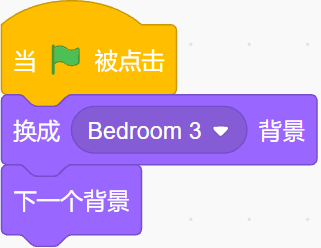
\includegraphics[width=.12\textwidth]{2a.png}
            \task 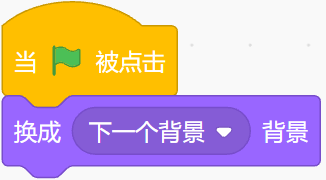
\includegraphics[width=.15\textwidth]{2b.png}
            \task 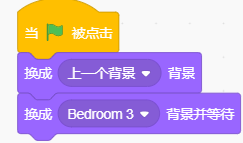
\includegraphics[width=.15\textwidth]{2c.png}
            \task 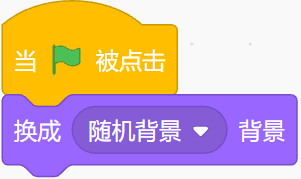
\includegraphics[width=.15\textwidth]{2d.png}
        \end{tasks}

        % 3
        \item 如下图所示,哪个程序可以切换成第4个背景?(\qquad)
        \begin{tasks}(4)
            \task 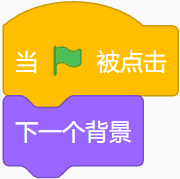
\includegraphics[width=.1\textwidth]{3a.png}
            \task 
\includegraphics[width=.15\textwidth]{3b.png}
            \task 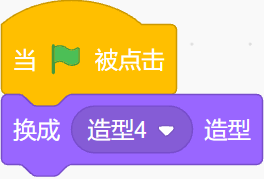
\includegraphics[width=.15\textwidth]{3c.png}
            \task 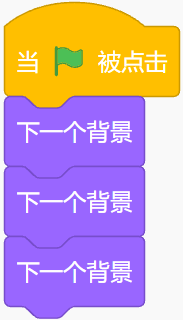
\includegraphics[width=.07\textwidth]{3d.png}
        \end{tasks}

        \begin{figure}[htbp]
            \centering
            \begin{minipage}[t]{.24\textwidth}
                \centering
                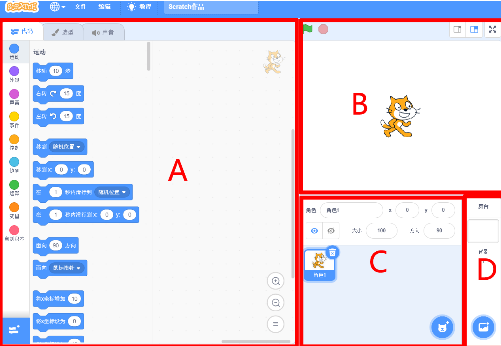
\includegraphics[width=1\textwidth]{1.png}
                \caption*{第1题}
            \end{minipage}
            \begin{minipage}[t]{.1\textwidth}
                \centering
                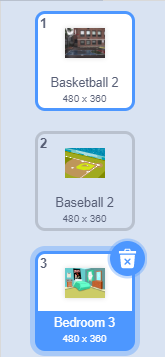
\includegraphics[width=\textwidth]{2.png}
                \caption*{第2题}
            \end{minipage}
            \begin{minipage}[t]{.09\textwidth}
                \centering
                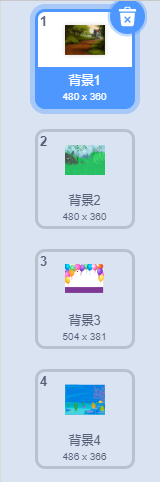
\includegraphics[width=\textwidth]{3.png}
                \caption*{第3题}
            \end{minipage}
            \begin{minipage}[t]{.2\textwidth}
                \centering
                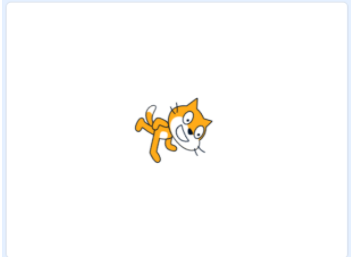
\includegraphics[width=\textwidth]{4.png}
                \caption*{第4题}
            \end{minipage}
            \begin{minipage}[t]{.2\textwidth}
                \centering
                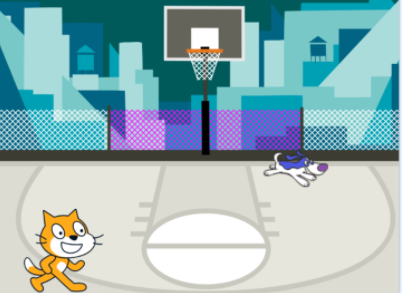
\includegraphics[width=\textwidth]{7.png}
                \caption*{第7题}
            \end{minipage}
        \end{figure}

        % 4
        \item 上图为小猫的初始方向,哪个积木可以让小猫面向正右方?(\qquad)
        \begin{tasks}(4)
            \task 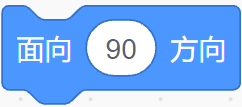
\includegraphics[width=.1\textwidth]{4a.png}
            \task 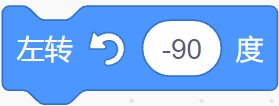
\includegraphics[width=.12\textwidth]{4b.png}
            \task 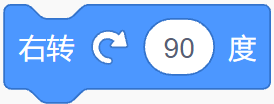
\includegraphics[width=.12\textwidth]{4c.png}
            \task 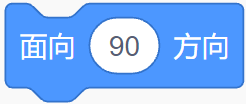
\includegraphics[width=.12\textwidth]{4d.png}
        \end{tasks}

        % 5
        \item 当我们要切换角色的造型时,需要用到下面哪个模块中的积木?(\qquad)
        \begin{tasks}(4)
            \task 
\includegraphics[width=.03\textwidth]{5a.png}
            \task 
\includegraphics[width=.03\textwidth]{5b.png}
            \task 
\includegraphics[width=.03\textwidth]{5c.png}
            \task 
\includegraphics[width=.03\textwidth]{5d.png}
        \end{tasks}

        % 6
        \item 下面哪个积木可以使小猫的面向方向由右转向左?(\qquad)
        \begin{tasks}(4)
            \task 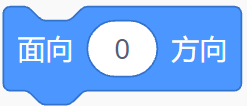
\includegraphics[width=.12\textwidth]{6a.png}
            \task 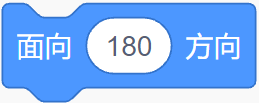
\includegraphics[width=.12\textwidth]{6b.png}
            \task 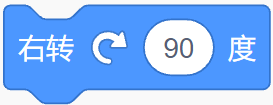
\includegraphics[width=.12\textwidth]{6c.png}
            \task 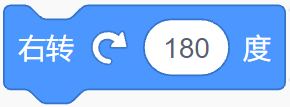
\includegraphics[width=.12\textwidth]{6d.png}
        \end{tasks}

        % 7
        \item 如上图,小猫在近处,小狗在远处,在不改变音量的情况下,使用哪个按钮,能让小狗叫的声音变小?(\qquad)
        \begin{tasks}(4)
            \task 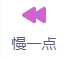
\includegraphics[width=.05\textwidth]{7a.png}
            \task 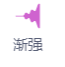
\includegraphics[width=.05\textwidth]{7b.png}
            \task 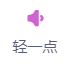
\includegraphics[width=.05\textwidth]{7c.png}
            \task 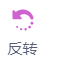
\includegraphics[width=.05\textwidth]{7d.png}
        \end{tasks}
           
        \newpage
        % 8
        \item 下面哪个积木可以使角色“说”一些内容,并且说的内容不会自动消失?(\qquad)
        \begin{tasks}(4)
            \task 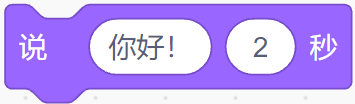
\includegraphics[width=.14\textwidth]{8a.png}
            \task 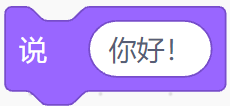
\includegraphics[width=.09\textwidth]{8b.png}
            \task 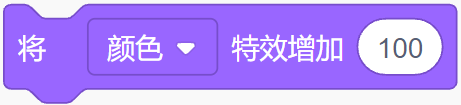
\includegraphics[width=.18\textwidth]{8c.png}
            \task 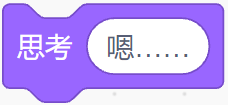
\includegraphics[width=.1\textwidth]{8d.png}
        \end{tasks}

        % 9
        \item 下面哪个积木可以使音调变高?(\qquad)
        \begin{tasks}(4)
            \task 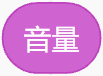
\includegraphics[width=.05\textwidth]{9a.png}
            \task 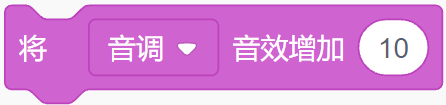
\includegraphics[width=.17\textwidth]{9b.png}
            \task 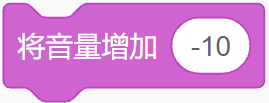
\includegraphics[width=.12\textwidth]{9c.png}
            \task 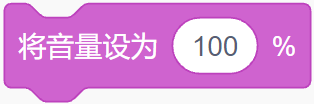
\includegraphics[width=.15\textwidth]{9d.png}
        \end{tasks}

       % 10
       \item 下图中哪个按钮可以添加新背景?(\qquad)
       \begin{tasks}(4)
           \task A
           \task B
           \task C
           \task D
       \end{tasks}

        % 11
        \item 执行下面哪段程序可以让小猫移到苹果所在的位置?(\qquad)
        \begin{tasks}(4)
            \task 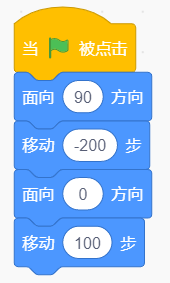
\includegraphics[width=.1\textwidth]{11a.png}
            \task 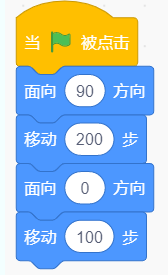
\includegraphics[width=.1\textwidth]{11b.png}
            \task 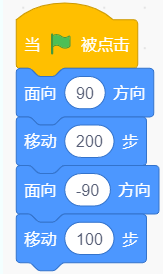
\includegraphics[width=.1\textwidth]{11c.png}
            \task 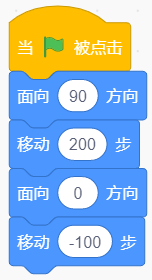
\includegraphics[width=.1\textwidth]{11d.png}
        \end{tasks}
        
        % 12
        \item 下面哪个积木可以使角色换成下一个造型?(\qquad)
        \begin{tasks}(4)
            \task 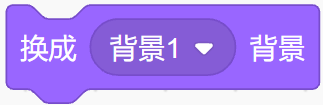
\includegraphics[width=.13\textwidth]{12a.png}
            \task 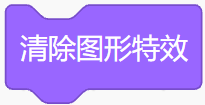
\includegraphics[width=.09\textwidth]{12b.png}
            \task 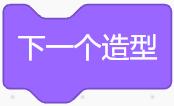
\includegraphics[width=.08\textwidth]{12c.png}
            \task 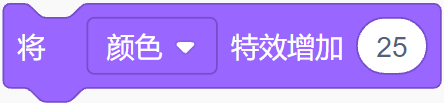
\includegraphics[width=.18\textwidth]{12d.png}
        \end{tasks}

        \begin{figure}[htbp]
            \centering
            \begin{minipage}[t]{.3\textwidth}
                \centering
                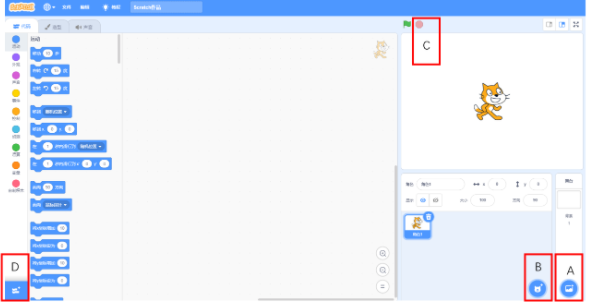
\includegraphics[width=\textwidth]{10.png}
                \caption*{第10题}
            \end{minipage}
            \begin{minipage}[t]{.2\textwidth}
                \centering
                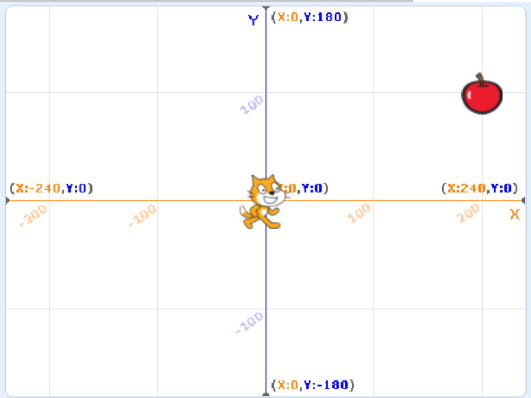
\includegraphics[width=\textwidth]{11.png}
                \caption*{第11题}
            \end{minipage}
            \begin{minipage}[t]{.45\textwidth}
                \centering
                \begin{minipage}[t]{.45\textwidth}
                    \centering
                    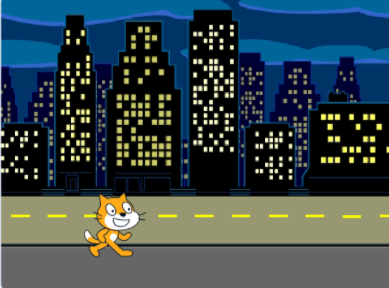
\includegraphics[width=\textwidth]{14-1.png}
                \end{minipage}
                \begin{minipage}[t]{.45\textwidth}
                    \centering
                    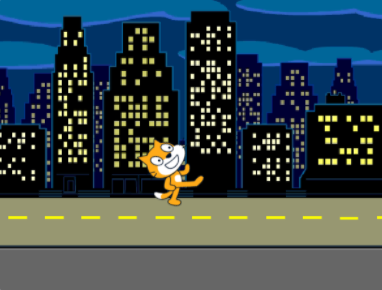
\includegraphics[width=\textwidth]{14-2.png}
                \end{minipage}
                \caption*{第14题}
            \end{minipage}
        \end{figure}

        % 13
        \item 下面哪个程序可以实现小猫一面唱歌一面左右摇摆?(\qquad)
        \begin{tasks}(4)
            \task 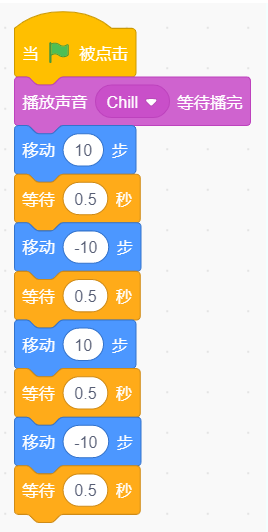
\includegraphics[width=.14\textwidth]{13a.png}
            \task \includegraphics[width=.1\textwidth]{13b.png}
            \task \includegraphics[width=.1\textwidth]{13c.png}
            \task \includegraphics[width=.12\textwidth]{13d.png}
        \end{tasks}

        % 14
        \item 上面左图为小猫初始位置,旋转方式为任意旋转,扶行下面哪段程序可以达到右图所示的效果?(\qquad)
        \begin{tasks}(4)
            \task \includegraphics[width=.08\textwidth]{14a.png}
            \task \includegraphics[width=.08\textwidth]{14b.png}
            \task \includegraphics[width=.08\textwidth]{14c.png}
            \task \includegraphics[width=.08\textwidth]{14d.png}
        \end{tasks}
    
        \newpage
        % 15
        \item 小猫有4个造型(依次为造型1,造型2,造型3,造型4),执行下图这段程序后,小猫的造型编号是?(\qquad)
        \begin{tasks}(4)
            \task 1
            \task 2
            \task 3
            \task 4
        \end{tasks}
        
        % 16
        \item 小明今年10岁,小亮说:“我比小明大2岁”。小红说:“我比小亮小4岁”。请问小红今年几岁?(\qquad)
        \begin{tasks}(4)
            \task 8
            \task 15
            \task 16
            \task 6
        \end{tasks}

        % 17
        \item 小明家住10楼,小明家上面还有8层,地下室有1层,请问包括地下室这栋楼一共多少层?(\qquad)
        \begin{tasks}(4)
            \task 16
            \task 18
            \task 10
            \task 19
        \end{tasks}

        % 18
        \item 下面哪个积木可以让角色切换到指定的一个造型?(\qquad)
        \begin{tasks}(4)
            \task \includegraphics[width=.13\textwidth]{18a.png}
            \task \includegraphics[width=.08\textwidth]{18b.png}
            \task \includegraphics[width=.08\textwidth]{18c.png}
            \task \includegraphics[width=.13\textwidth]{18d.png}
        \end{tasks}

        % 19
        \item 执行下面程序,小猫共走了多少步?(\qquad)
        \begin{tasks}(4)
            \task 115
            \task 100
            \task 110
            \task 200
        \end{tasks}

        % 20
        \item 找规律:1,3,4,7,(\quad),18,请问()应该填哪个数字?(\qquad)
        \begin{tasks}(4)
            \task 15
            \task 12
            \task 11
            \task 17
        \end{tasks}

        % 21
        \item 默认小猫角色,不改变造型,下面哪组积木可以实现小猫倒立?(\qquad)
        \begin{tasks}(4)
            \task \includegraphics[width=.15\textwidth]{21a.png}
            \task \includegraphics[width=.15\textwidth]{21b.png}
            \task \includegraphics[width=.15\textwidth]{21c.png}
            \task \includegraphics[width=.15\textwidth]{21d.png}
        \end{tasks}

        \begin{figure}[htbp]
            \centering
            \begin{minipage}[t]{.18\textwidth}
                \centering
                \includegraphics[width=\textwidth]{15.png}
                \caption*{第15题}
            \end{minipage}
            \begin{minipage}[t]{.15\textwidth}
                \centering
                \includegraphics[width=.7\textwidth]{19.png}
                \caption*{第19题}
            \end{minipage}
            \begin{minipage}[t]{.2\textwidth}
                \centering
                \includegraphics[width=\textwidth]{21.png}
                \caption*{第21题}
            \end{minipage}
        \end{figure}

        % 22
        \item 角色小猫默认的音量是多大?(\qquad)
        \begin{tasks}(4)
            \task 0
            \task 100
            \task 50
            \task 200
        \end{tasks}

        % 23
        \item 同学们站成一排,从左边数小明是第5人,从右边数小明是第5人,请问这排共多少学生?(\qquad)
        \begin{tasks}(4)
            \task 5
            \task 8
            \task 9
            \task 10
        \end{tasks}

        % 24
        \item 小猫有4个造型(依次为造型1、造型2、造型3、造型4),现在默认是造型2,下面哪段程序,可以将小猫变成造型1?(\qquad)
        \begin{tasks}(4)
            \task \includegraphics[width=.1\textwidth]{24a.png}
            \task \includegraphics[width=.1\textwidth]{24b.png}
            \task \includegraphics[width=.07\textwidth]{24c.png}
            \task \includegraphics[width=.07\textwidth]{24d.png}
        \end{tasks} 
        
        % 25
        \item 下面哪组积木可以让小猫最终面向100度?(\qquad)
        \begin{tasks}(4)
            \task \includegraphics[width=.1\textwidth]{25a.png}
            \task \includegraphics[width=.1\textwidth]{25b.png}
            \task \includegraphics[width=.1\textwidth]{25c.png}
            \task \includegraphics[width=.1\textwidth]{25d.png}
        \end{tasks}
    \end{enumerate}

    {\noindent\heiti 第二部分、判断题(共 10 题,每题 2 分,共20分.)}
    \begin{enumerate}
        \setcounter{enumi}{25}
        % 26
        \item 只能使用\includegraphics[width=.15\textwidth]{26.png}积木实现背景切折.(\qquad)

        %27
        \item 小狗的造型如下图所示,执行下面程序,可以看到小狗吐舌头奔跑的动画.(\qquad)
        
        %28
        \item 使用\includegraphics[width=.1\textwidth]{28.png}积木可以实现随机切换造型.(\qquad)
  
        %29
        \item 有一段绳子,在绳子中间剪了3刀,最后绳子被分成了3段.(\qquad)
        
        %30
        \item 使用\includegraphics[width=.15\textwidth]{30.png}积木可以让音量变小.(\qquad)

        %31
        \item 点击下图所示按钮,可以添加角色.(\qquad)
        
        \begin{figure}[htbp]
            \centering
            \begin{minipage}[t]{.23\textwidth}
                \centering
                \begin{minipage}[t]{.45\textwidth}
                    \centering
                    \includegraphics[width=\textwidth]{27-1.png}
                \end{minipage}
                \begin{minipage}[t]{.45\textwidth}
                    \centering
                    \includegraphics[width=\textwidth]{27-2.png}
                \end{minipage}
                \caption*{第27题}
            \end{minipage}
            \begin{minipage}[t]{.3\textwidth}
                \centering
                \includegraphics[width=\textwidth]{31.png}
                \caption*{第31题}
            \end{minipage}
            \begin{minipage}[t]{.25\textwidth}
                \centering
                \includegraphics[width=\textwidth]{32.png}
                \caption*{第32题}
            \end{minipage}
            \begin{minipage}[t]{.15\textwidth}
                \centering
                \includegraphics[width=\textwidth]{35.png}
                \caption*{第35题}
            \end{minipage}
        \end{figure}
        
        %32
        \item 可以改变上图中“大小”的数值来调节角色大小,目前“大小”数值为“100”,是最大值,不能再变大了.(\qquad)
        
        %33
        \item 在声音编辑器中,点击\includegraphics[width=.08\textwidth]{33.png}按钮能够使声音反转.(\qquad)
        
        %34
        \item 默认小猫角色,不改变造型,\includegraphics[width=.15\textwidth]{34.png}积木可以让角色面向左.(\qquad)
        
        %35
        \item 执行上图程序,角色回到位置$(x:-150,y:-120)$.(\qquad)
    \end{enumerate}

    \newpage
    {\noindent\heiti 第三部分、编程题(共 2 题,共30分.)}
    \begin{enumerate}
        \setcounter{enumi}{35}
        
        % 36
        \item 海底世界:
        
        1. 准备工作
        \begin{tasks}[label = (\arabic*)]
            \task 背景:Underwater1;
            \task 角色:Fish、Starfish.
        \end{tasks}
        2. 功能实现
        \begin{tasks}[label = (\arabic*)]
            \task 如右图所示设置Fish初始位置为舞台上方的左侧,面向右;设置Starfish初始位置 在舞台左下方;
            \task 点击绿旗Fish先说“你好!”2秒后,Starfish说“你好!”2秒;
            \task Fish一直游到舞台边缘,碰到边缘时就往回走,注意肚皮不能朝上;
            \task Starfish不动,每过0.5秒切换一次造型;
            \task 添加背景音乐“Bubbles”,播放背景音乐.
        \end{tasks}
        \begin{figure}[htbp]
            \centering
            \includegraphics[width=.2\textwidth]{36.png}
        \end{figure}
            
        %37
        \item 小猫当裁判:
        
        1. 准备工作
        \begin{tasks}[label = (\arabic*)]
            \task 背景:School、Soccer2;
            \task 角色:小猫.
        \end{tasks}
        2. 功能实现
        \begin{tasks}[label = (\arabic*)]
            \task 设置小猫初始位置如下图所示,初始方向为右;
            \task 设置初始背景为School;
            \task 点击绿旗,等待1秒后,小猫面向学校,走到学校门口,切换背景Soccer2;
            \task 切换成Soccer2后,小猫位置在左下角;
            \task 小猫进入Soccer2,播放声音Goal Cheer;
            \task 调整小猫面向方向,朝着右上角的小红旗走去,最后停在小红旗处.
        \end{tasks}

        \begin{figure}[htb]
            \begin{minipage}[t]{.23\textwidth}
                \centering
                \includegraphics[width=\textwidth]{37-1.png}
            \end{minipage}
            \begin{minipage}[t]{.23\textwidth}
                \centering
                \includegraphics[width=\textwidth]{37-2.png}
            \end{minipage}
            \begin{minipage}[t]{.23\textwidth}
                \centering
                \includegraphics[width=\textwidth]{37-3.png}
            \end{minipage}
            \begin{minipage}[t]{.23\textwidth}
                \centering
                \includegraphics[width=\textwidth]{37-4.png}
            \end{minipage}
        \end{figure}
    \end{enumerate}
\end{document}